\subsection{Исследование существования циклов длины 2 и 3}

\begin{definition}\label{def:cycle}
        Пусть дана система $u_{t+1} = f(u_t)$. Множество точек $u_1,\; u_2,\;\dots,\; u_k$, являющиеся траекторией системы, образуют цикл, если
        $$
                u_2 = f(u_1),\; u_3 = f(u_2),\;\dots,\;u_k = f(u_{k-1}),\; u_1 = f(u_k).
        $$
        \cite[стр.~87]{bratus10}
\end{definition}
\textit{Замечание.} Любая неподвижная точка цикла является неподвижной точкой отображения $f^{(k)}(u) = \underbrace{f(f(\dots f(f}_k (u))\dots))$.
            
\begin{definition}
        Будем говорить, что~все натуральные числа упорядочены по~Шарковскому, если
        $$
                \begin{array}{ll}
                        3 \succ 5 \succ 7 \succ \ldots \succ & \textrm{все нечетные числа, кроме $1$}\\
                        \succ 2 \cdot 3 \succ 2 \cdot 5 \succ 2 \cdot 7 \succ \ldots \succ & \textrm{все нечетные числа, умноженные на $2$, кроме $1$} \\
                        \succ 2^2 \cdot 3 \succ 2^2 \cdot 5 \succ 2^2 \cdot 7 \succ \ldots \succ & \textrm{все нечетные числа, умноженные на $2^2$, кроме $1$} \\
                        \succ 2^3 \cdot 3 \succ 2^3 \cdot 5 \succ 2^3 \cdot 7 \succ \ldots \succ & \textrm{все нечетные числа, умноженные на $2^3$, кроме $1$} \\
                        \succ \ldots \succ\\
                        \succ \ldots \succ 2^3 \succ 2^2 \succ 2 \succ 1.
                \end{array}
        $$
        \cite[стр.~88]{bratus10}
\end{definition}

\begin{theorem}[Шарковского]
        Пусть $f:\R\rightarrow\R$~--- непрерывное отображение, и~пусть $f$ имеет цикл длины $k$. Тогда $f$ имеет цикл длины $m$ для~всех таких $m$, что $k \succ m$ в~указанном выше порядке. \cite[стр.~89]{bratus10}
\end{theorem}
\textit{Замечание.} Из~теоремы непосредственно следует, что:
\begin{enumerate}
        \item если отображение имеет цикл длины~3, то~существует цикл любой длины (\textit{хаос});
        \item если отображение не~имеет цикла длины~2, то~оно не~имеет никаких циклов.
\end{enumerate}
\textit{Замечание.} Из определения~\ref{def:cycle} следует, что для~нахождения цикла длины $k$ нужно найти решение системы
$$
        \left\{
        \begin{array}{ll}
                f^{(k)}(u) &=u \\
                \frac{df^{(k)}(u)}{du} &=1.
        \end{array}
        \right.
$$

По бифуркационной диаграмме наглядно видно, что при $r$ равном, например, 7 в системе возникает цикл длины 2. Вообще говоря, по диаграмме нельзя формулировать строгих утверждений, так как она построена с учётом погрешностей вычислений, но она позволяет нам существенно сократить подозрительную область изменения параметра, в которой возникает цикл нужной нам длины. Поэтому для нахождения цикла длины 2 функции $f(u) = ru^2e^{-u}$ системы~\ref{eq:first_discrete_system} при $7 \leqslant r \leqslant 8$ решим систему 
$$
        \left\{
        \begin{array}{ll}
                f^{(2)}(u) &=u \\
                \frac{df^{(2)}(u)}{du} &=1.
        \end{array}
        \right.
$$

Рассмотрим значения параметра $r = 7,5$. Из рисунка \ref{img:one_step_cycle2_system} видно, что имеются три потенциальные точки (точки пересечения графиков, близкие к нулю), которые могут образовать цикл.
\begin{figure}[h]
        \centering
        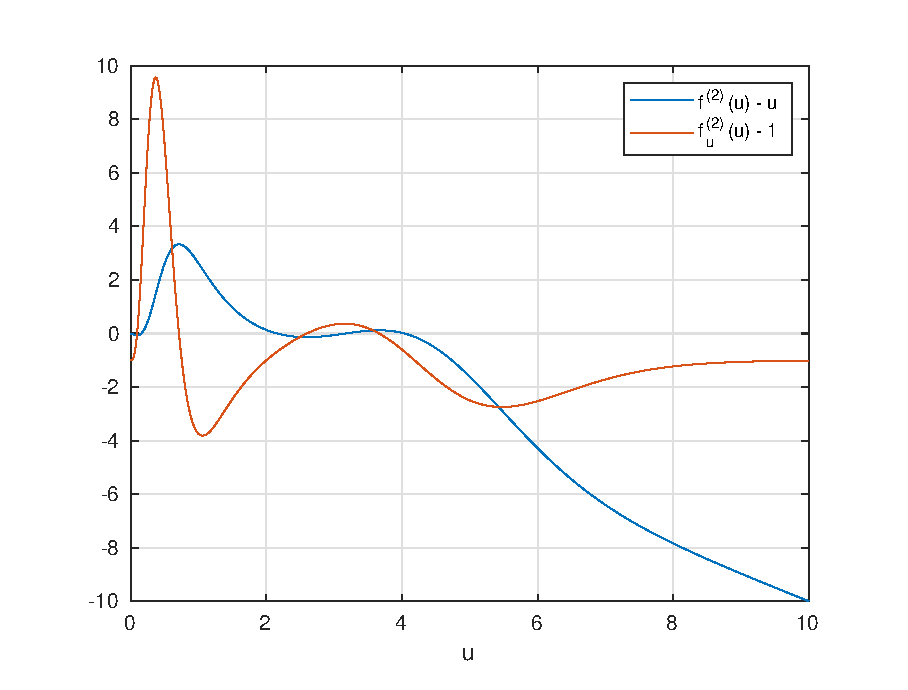
\includegraphics[width=0.8\linewidth]{img/one_step_cycle2_system.eps}
        \caption{Поиск цикла длины 2 при $r = 7,5$.}
        \label{img:one_step_cycle2_system}
\end{figure}
Возьмем за начальное приближение одну из этих точек (Рис.~\ref{img:one_step_cycle2_search}). Видно, что траектория стремится к циклу. Действительно, выбрав $u_0 \approx 2,164$, отчетливо прослеживается цикл длины 2 (Рис.~\ref{img:one_step_cycle2_total}).
\begin{figure}[h]
        \centering
        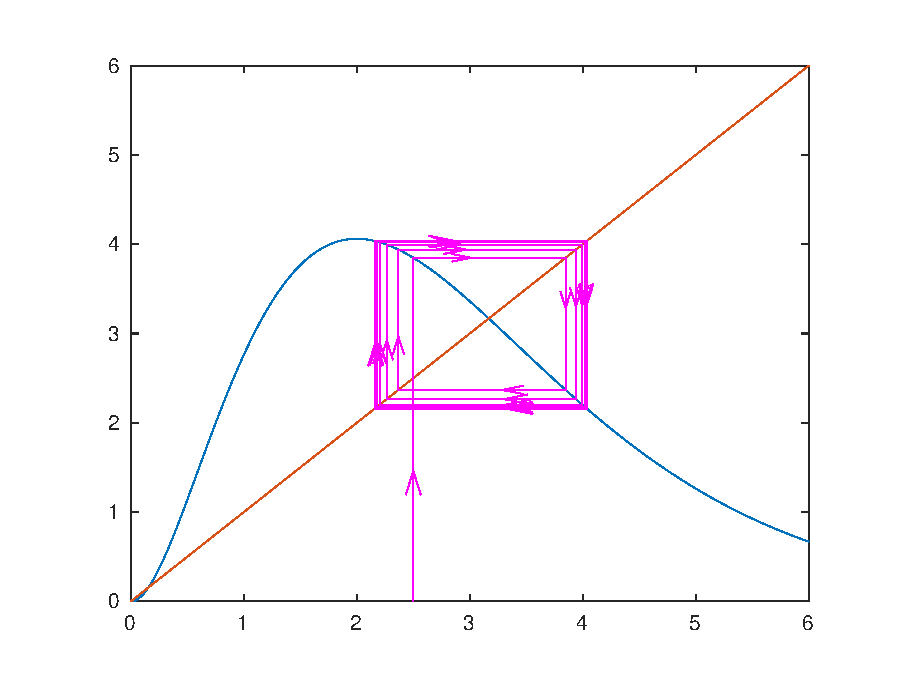
\includegraphics[width=0.8\linewidth]{img/one_step_cycle2_search.eps}
        \caption{Траектория при начальном приближении $u_0 = 2,5$. $r = 7,5$.}
        \label{img:one_step_cycle2_search}
\end{figure} 
\begin{figure}[h]
        \centering
        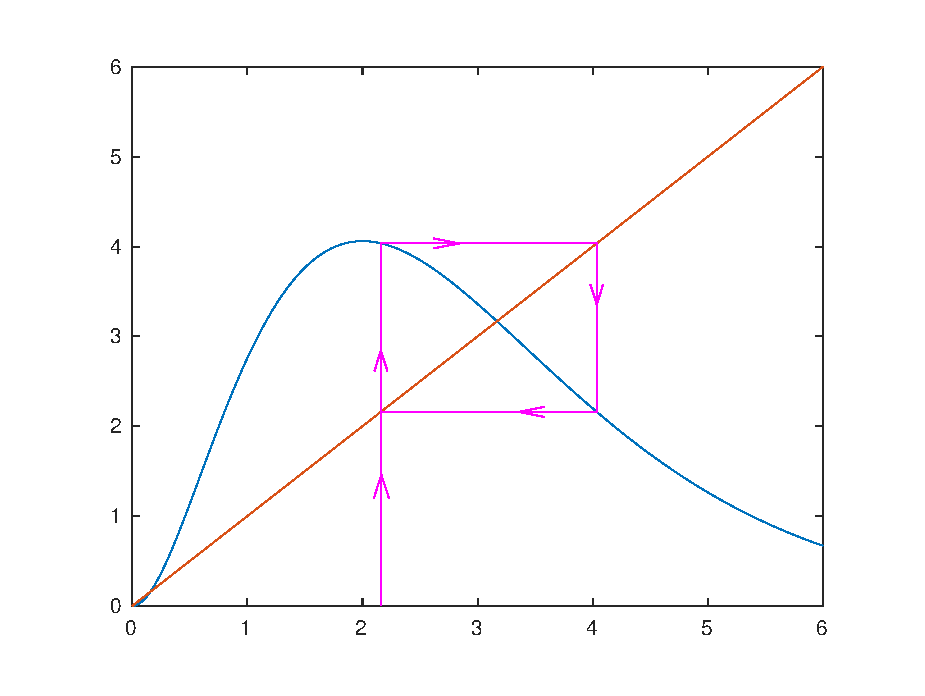
\includegraphics[width=0.8\linewidth]{img/one_step_cycle2_total.eps}
        \caption{Траектория при начальном приближении $u_0 = 2,164$. $r = 7,5$.}
        \label{img:one_step_cycle2_total}
\end{figure}

Теперь можно задаться вопросом существования цикла длины 3. Из бифуркационной диаграммы видно, что если цикл длины 3 существует, то искать его лучше при $13,5 \leqslant r \leqslant 13,6$. Аналогично рассуждениям для цикла длины два, цикл длины 3 можно получить при $r = 13,6$ при начальном приближении $u_0 = 1,9$ (Рис.~\ref{img:one_step_cycle3}).

\begin{figure}[h]
        \centering
        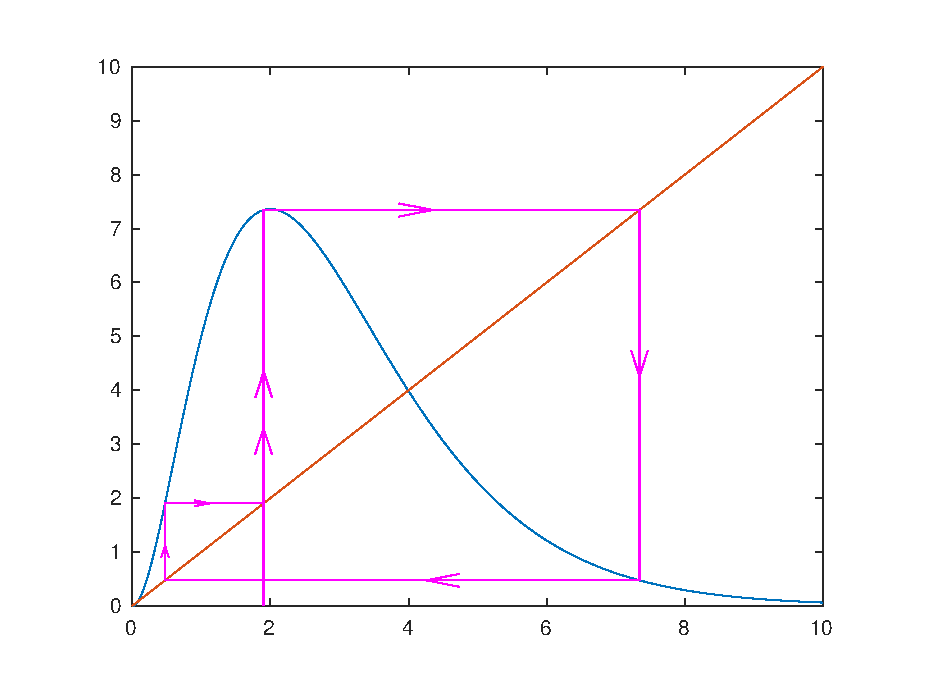
\includegraphics[width=0.8\linewidth]{img/one_step_cycle3.eps}
        \caption{Траектория при начальном приближении $u_0 = 1,9$. $r = 13,6$.}
        \label{img:one_step_cycle3}
\end{figure}